\documentclass{article}
\usepackage{amsmath}
\usepackage{amssymb}
\usepackage{amsthm}
\usepackage{thmtools}
\usepackage{cases}
\usepackage{enumitem}
\usepackage{xcolor}
\usepackage{cancel}
\usepackage{cite}
\usepackage{graphicx}
\usepackage{float}
\usepackage{array}
\usepackage{multirow}

\usepackage{algorithm2e}
\RestyleAlgo{ruled}
\SetKwComment{Comment}{/* }{ */}

\usepackage{geometry}
\geometry{margin=4cm, vmargin=3cm}

\setlength\parindent{0pt}

\usepackage{mathtools}
\newcommand{\expect}{\operatorname{E}\expectarg}
\DeclarePairedDelimiterX{\expectarg}[1]{[}{]}{%
  \ifnum\currentgrouptype=16 \else\begingroup\fi
  \activatebar#1
  \ifnum\currentgrouptype=16 \else\endgroup\fi
}

\newcommand{\innermid}{\nonscript\;\delimsize\vert\nonscript\;}
\newcommand{\activatebar}{%
  \begingroup\lccode`\~=`\|
  \lowercase{\endgroup\let~}\innermid 
  \mathcode`|=\string"8000
}

\title{Asian options pricing}
\author{David Castro \qquad Maxime Leroy}
\date{15 Januray 2024}

\begin{document}
\maketitle

\section*{Introduction}

An Asian option is any option with payoff of the form:
\[
	\left( S_t \right)_{t \in [0, T]} \mapsto g \left( S_T, A_T \right) \quad \text{with} \quad A_T := \frac{1}{T} \int_0^T S_u du
\]
where $\left( S_t \right)_t$ denotes the trajectory of the underlying and $T$ is the maturity of the option.
For instance, a \textit{fixed-strike} Asian call has $g(x, a) := e^{-rT} \left[ a - K \right]_+$ where $K$ denotes the strike
and a \textit{floatting-strike} Asian call has $g(s, a) := e^{-rT}  \left[ s - a \right]_+$.
In the first case, the option is exercised by its owner
if the underlying has lied above the strike \textbf{on average} throughout its lifetime. In the second case,
it is worth exercising it when the underlying is above its average value at expiry.

\

This work studies different pricing techniques for Asian options and will tackle \textbf{only fixed-strike Asian calls}
for simplicity. Furthermore, we will use Black-Scholes model. In that context, simulating $S_T$ is straightforward
and the real challenge consists in simulating $A_T$. That is why our developments for fixed-strike Asian calls
adapt directly to any Asian option of the form given above.

\

We first introduce and implement different Monte-Carlo approaches as developed by Lambert et al. \cite{main}
and B. Bouchard \cite{Bouchard}. We then compare them with a PDE approach as presented by
Rogers et al. \cite{Rogers}.

\section*{Assumptions and notations}

We consider the case of an arbitrage-free complete market and note $\mathbb Q$ the corresponding
risk-neutral measure. Therefore, the true price of the option is given by:
\[
	C := e^{-rT} \mathbb E_{\mathbb Q} \left[ [ A_T - K ]_+ \right]
\]
where $r$ is the risk-free interest rate, assumed to be constant.
As specified above, we also use Black-Scholes model, which yields:
\begin{equation}
	\forall t \in [0, T], \ S_t = S_0 \exp \left\{ \left( r - \frac{\sigma^2}{2} \right) t + \sigma W_t \right\}
	\tag{BS}
\end{equation}
where $W := (W_t)_{t \in [0, T]}$ denotes a Wiener process under $\mathbb Q$.

\

In the context of Monte-Carlo methods, we call \textbf{a scheme} a random variable $\bar A_T$ made to approximate
the quantity $A_T$ for a given set of parameters. Therefore, provided $\{ \bar A_T^i \}_{i = 1, \dots, n}$ are
independent and identically distributed (i.i.d.) copies of $\bar A_T$, the Monte-Carlo estimate of the fixed-strike
Asian call we get is:
\[
	\theta_n := e^{-rT} \sum_{i=1}^n \left[ \bar A_T^i - K \right]_+ \xrightarrow[n \to \infty]{\mathbb P}
	e^{-rT} \mathbb E_{\mathbb Q} \left[ [ \bar A_T - K ]_+ \right]
\]

For $m \in \mathbb N^*$ time steps, we note:
\begin{itemize}[label=$\cdot$]
\item $t_0, \dots, t_m$ the regular subdivision of $[0, T]$, whose mesh is thus $h = \frac{T}{m}$.
\item $\bar W_{t_0}^m, \dots, \bar W_{t_m}^m$ a realization of $W$ at these time steps.
\item $\bar S_{t_0}^m, \dots, \bar S_{t_m}^m$ the corresponding realization of the underlying, obtained
	with (BS).
\item $\mathcal B_h$ the $\sigma$-field generated by $\left\{ S_{t_0}, \dots, S_{t_m} \right\}$.
\end{itemize}

\section{Naive approach}

The most basic Monte-Carlo approach to the problem consists in approximating the integral
of the underlying over its trajectory by a Riemann sum. This is our first scheme:
\begin{equation}
	A_T \approx \bar A_T^{r, m} := \frac{h}{T} \sum_{k=0}^{m-1} \bar S_{t_k}^m
	= \frac{1}{m} \sum_{k=0}^{m-1} \bar S_{t_k}^m 
	\tag{1}
\end{equation}

Figure 1 shows the result
of this method for different values of $K$, $T$ and $\sigma$ where we took $n =10,000$ and $m=100$.
One can already notice that it tallies with the common idea that Asian calls are cheaper than European calls
for a given set of parameters. Also, quite intuitively, the gap widens when $\sigma$ and $T$ grow: the smaller
both of them are, the closer to the initial value the underlying will remain, leading to $A_T \approx S_T \approx S_0$
on average.

\begin{figure}[H]
  \hspace*{-0.02\linewidth}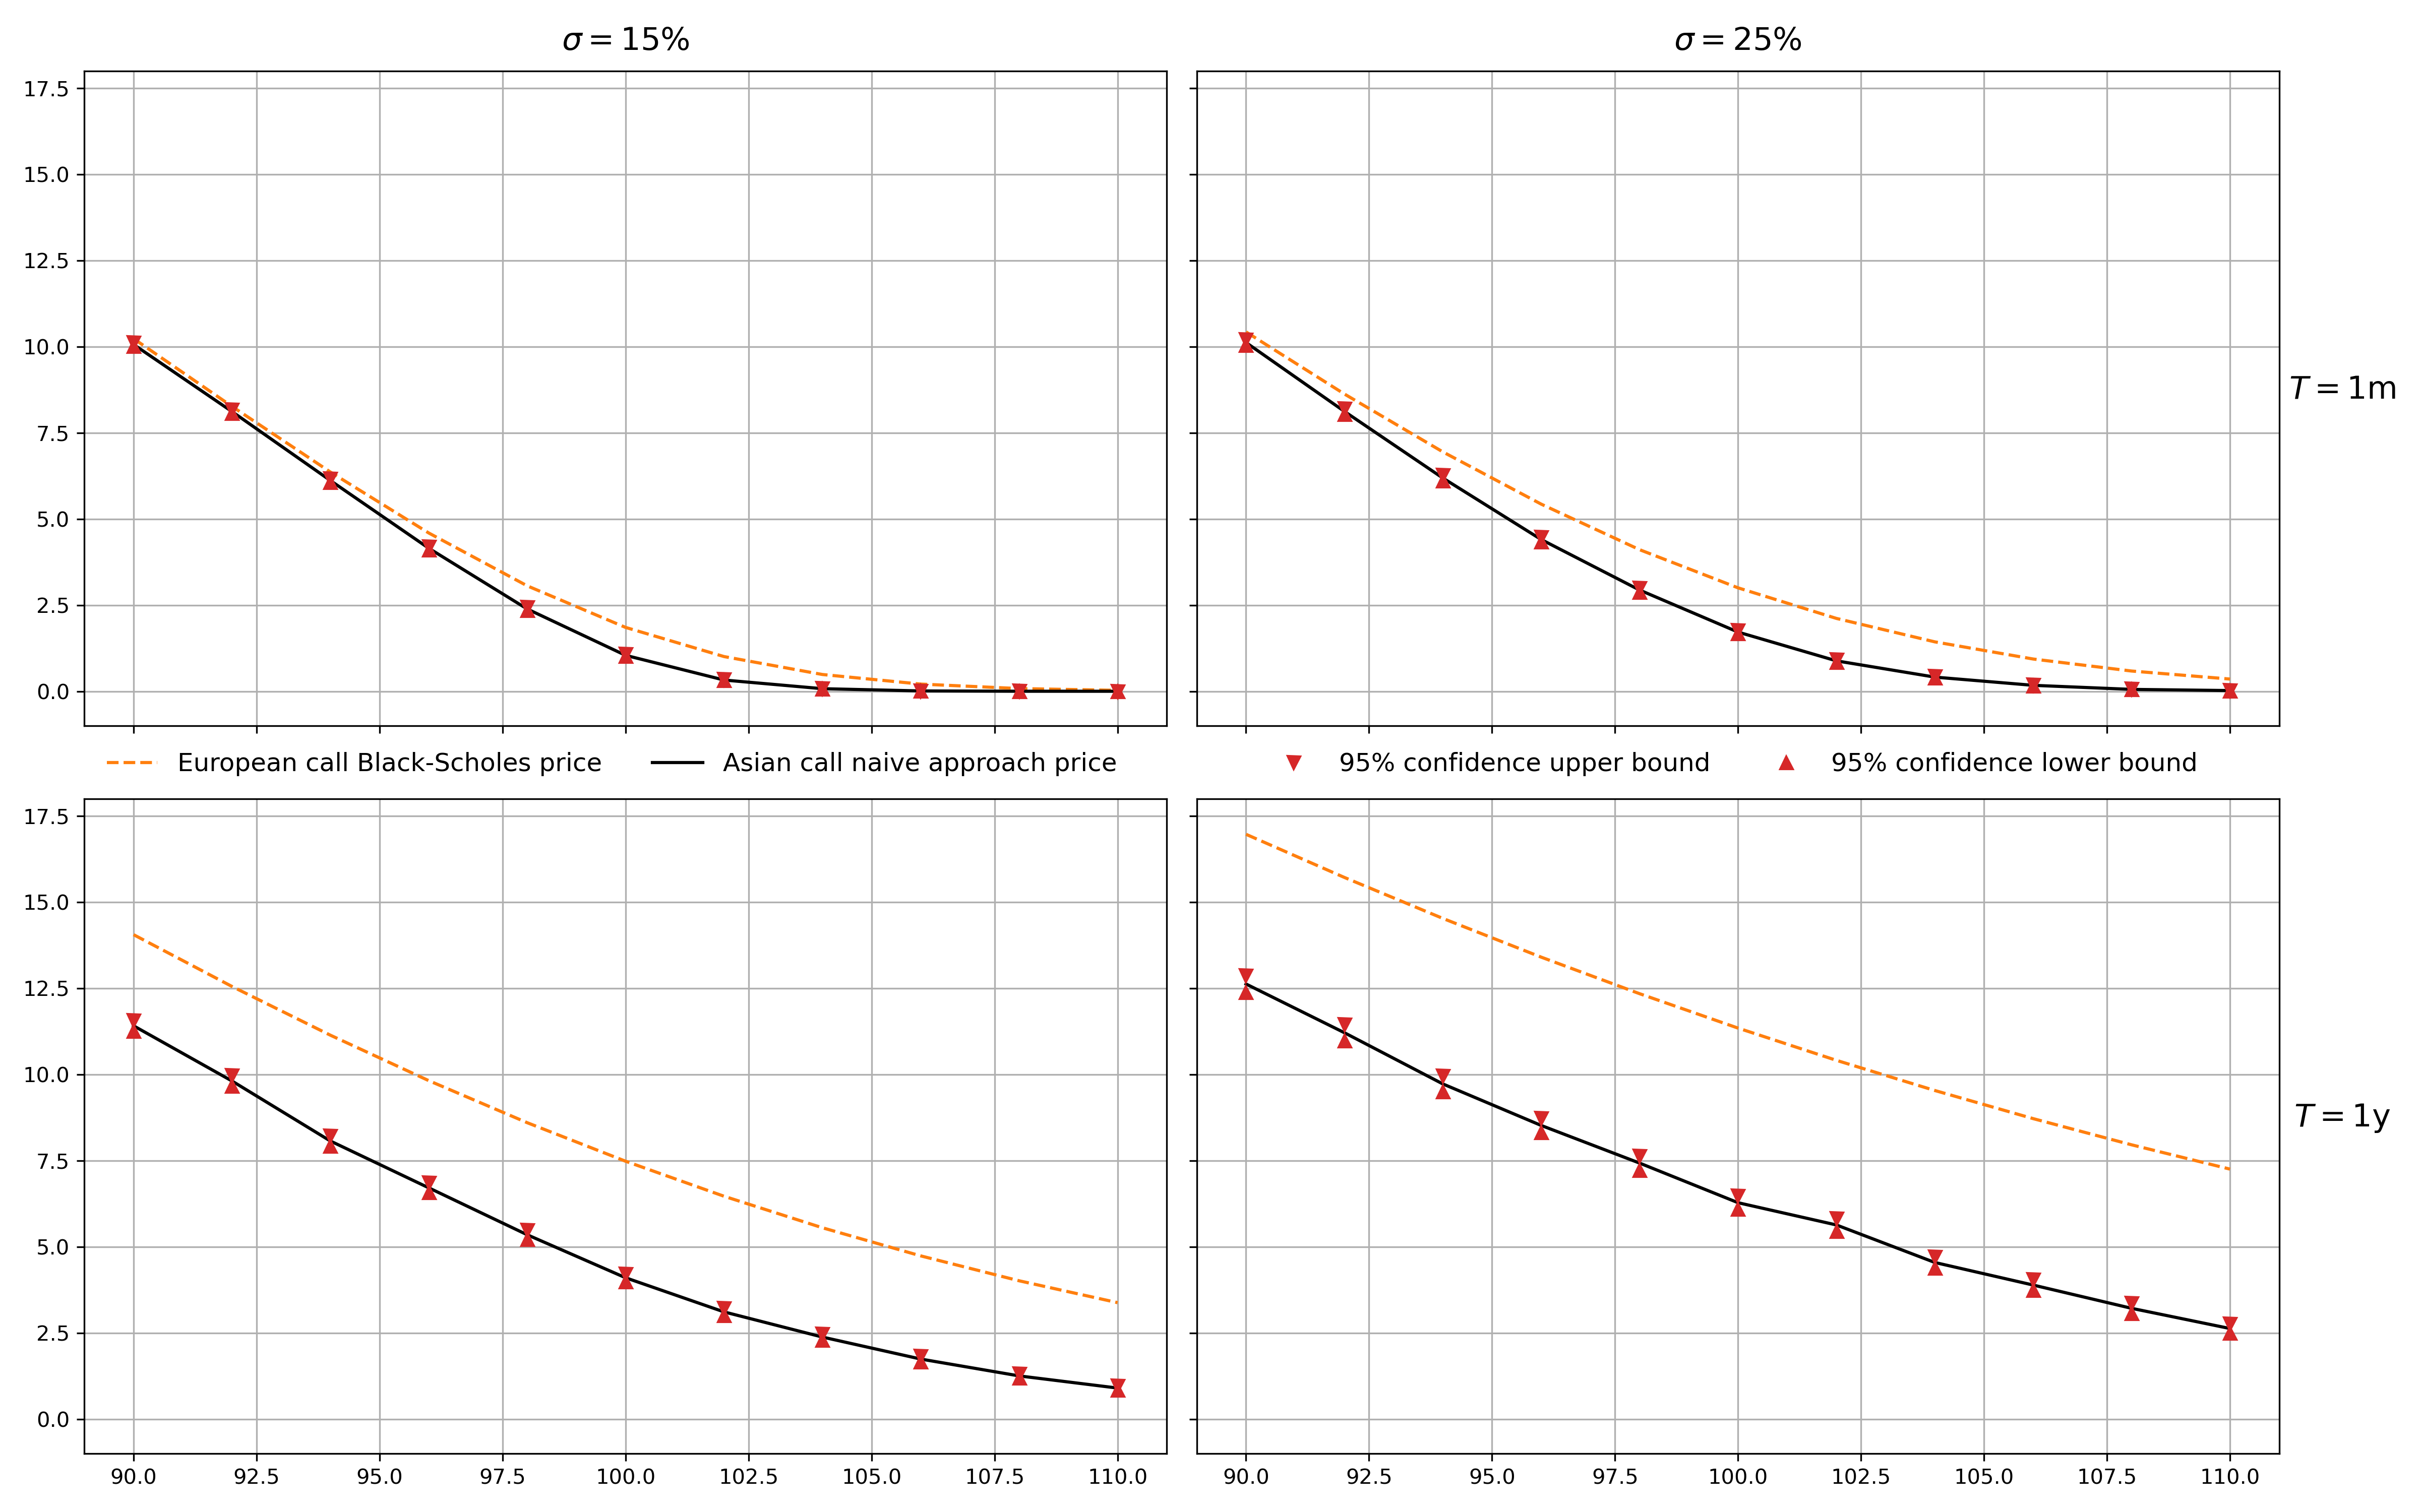
\includegraphics[width=1.065\textwidth]{charts/prices.png}
  \caption{Fixed-strike Asian call naive pricing for different values of $K$, $\sigma$ and $T$}
\end{figure}

However, these charts, particularly the one for $\sigma = 25\%$ and $T=1$y, reveal some fluctuations with
a greater magnitude than the length of the $95\%$ confidence intervals plotted in red. This stems from the bias
introduced by the approximation of $A_T$. This seems to be the main flaw of the
naive approach: even if the variance already looks satisfactory, the bias increases rapidly with the parameters, which
yields imprecise results.

\

The following models all give similar charts. In the below, we rather focus on the graphical representation
of the convergence properties of each scheme. As suggested in the previous paragraph, this is
the main challenge that the following approaches mean to address.

\section{Improved Monte-Carlo approaches}
\subsection{Two finer approximations}

A first improvement of the above approach proposes to better use the information provided by the simulation
$\bar S_0^m, \bar S_{t_1}^m, \dots, \bar S_T^m$ to approximate the integral $A_T$.
It relies on the fact that once the trajectory has been simulated, the best estimation of the price is:
\[
	\bar C^m := e^{-rT} \mathbb E \left[ \left[ A_T - K \right]_+ \mid \mathcal B_h \right]
\]

By the tower property, the expectation (estimated by a Monte-Carlo method with $n$ trajectories)
of this conditional expectation is the price of the Asian call.
At this stage, this quantity is not known either. \cite{main} introduces the following simplification (S):

\begin{align}
	\bar C^m &\approx e^{-rT}  \bigl[ \mathbb E \left[A_T
		\ \vert \ \mathcal B_h \right] - K \bigr]_+
	\tag{S} \\
	&= e^{-rT} \left[ \frac{1}{T}\sum_{k=0}^{m-1} \mathbb E \left[ \int_{t_k}^{t_{k+1}} S_u du
		\ \Big\vert \ \mathcal B_h \right] - K \right]_+
	\notag \\
	&= e^{-rT} \left[ \frac{1}{T}\sum_{k=0}^{m-1} \int_{t_k}^{t_{k+1}} \mathbb E \left[ S_u
		\ \big\vert \ \mathcal B_h \right] du - K \right]_+
	\notag \\
	&= e^{-rT} \left[ \frac{1}{T}\sum_{k=0}^{m-1} \bar S_{t_k}^m \int_{t_k}^{t_{k+1}}
		\mathbb E \left[ e^{\left( r - \frac{\sigma^2}{2} \right) (u - t_k) + \sigma \left( W_t - W_{t_k} \right)}
		\ \big\vert \ \mathcal B_h \right] du - K \right]_+
	\notag
\end{align}

We need to further simplify this expression. Let us considere the function $f$ defined as:
\[
	f : (t, w) \mapsto \exp \left\{ \left( r - \frac{\sigma^2}{2} \right) t + \sigma w \right\}
\]
A first-order Taylor expansion gives (by It\^o's lemma):
\[
	f(t, W_t) \underset{t \to 0}{\approx} 1 + \partial_t f(0, 0) t + \partial_w f(0, 0) W_t
	+ \frac{1}{2} \partial_{ww}^2 f (0, 0) t = 1 + rt + \sigma W_t
\]

It leads to the additional approximation below for all $k \in \{ 0, \dots, m - 1 \}$:
\[
	\int_{t_k}^{t_{k+1}} \mathbb E \left[ S_u \mid \mathcal B_h \right] du
	\approx \bar S_{t_k}^m \int_{t_k}^{t_{k+1}}
		\mathbb E \left[ 1 + r (u - t_k) + \sigma \left( W_t - W_{t_k} \right)
		\ \big\vert \ \mathcal B_h \right] du
\]

Finally, the process
$\left\{ \left( W_u \mid \bar W_{t_k}^m, \bar W_{t_{k+1}}^m \right) ; u \in [t_k, t_{k + 1}] \right\}$
follows a Brownian bridge, which allows
to compute the expectation and then the integral and yields the following scheme:

\begin{equation}
    A_T \approx \bar A_T^{e, m} = \frac{1}{m} \sum_{k=0}^{m-1} \bar S_{t_k}^m
    	\left( 1 + \frac{rh}{2} + \sigma \frac{\bar W_{t_{k+1}}^m - \bar W_{t_k}^m}{2} \right) \tag{2}
\end{equation}

The above development is actually equivalent to a trapezoidal method in comparison with the more
basic Riemann sum used in scheme $(1)$.

\

Instead of simplification (S), \cite{Bouchard} and \cite{main} suggest a quite similar approach. For each step
of the Monte-Carlo estimation, first fix a trajectory with the explicit formula given by Black-Scholes model
(same as before). Then, rather than computing the conditional expectation $\bar C^m$, simulate a realization of
$e^{-rT} \left[ A_T - K \right]_+$ conditionally to the trajectory. Similarly:
\begin{align*}
	\int_{t_k}^{t_{k+1}} S_u du
	&\approx
	S_{t_k} \int_{t_k}^{t_{k+1}} \left\{ 1 + r (u - t_k) + \sigma \left( W_u - W_{t_k} \right) \right\} du \\
	&= h S_{t_k} \left\{ 1 + \frac{rh}{2} + \frac{\sigma}{h} \int_{t_k}^{t_{k+1}} \left( W_u - W_{t_k} \right) du \right\}
\end{align*}

Furthermore, the remaining integral of the increment of the Brownian Motion is a Gaussian variable and we can
compute its expectation and variance conditionally to the trajectory since the integrand follows a Brownian Bridge.
Thus, we can indeed simulate it as stated above. In the following, we note:
\[
	\bar I_k^m := \left( \frac{1}{h}
	\int_{t_k}^{t_{k+1}} \left( W_u - W_{t_k} \right) du \ \Big\vert \ \mathcal B_h
	\right)
\]

In short, $\bar I_k^m \sim \mathcal N(\mu_k, \sigma_k^2)$ with the following parameters:
\begin{align*}
	\mu_k
	&= \frac{1}{h} \int_{t_k}^{t_{k+1}} \mathbb E \left[ W_u - W_{t_k} \mid \bar W_{t_{k+1}}^m, \bar W_{t_k}^m \right] du \\
	&= \frac{1}{h} \left( \bar W_{t_{k+1}}^m - \bar W_{t_k}^m \right) \int_{t_k}^{t_{k+1}} \frac{u - t_k}{t_{k+1} - t_k} du \\
	&= \frac{1}{2} \left( \bar W_{t_{k+1}}^m - \bar W_{t_k}^m \right)
\end{align*}
Interchanging the conditional expectation and the integrals yields:
\[
	\sigma_k^2 = \frac{1}{h^2} \int_{t_k}^{t_{k+1}} \int_{t_k}^{t_{k+1}}
		\mathrm{Cov} \left( W_u, W_v \mid \bar W_{t_{k+1}}^m, \bar W_{t_k}^m \right) du dv 
\]

\noindent Then, by symmetry of the covariance, we have:
\begin{align*}
	\sigma_k^2 &= \frac{2}{h^2} \int_{t_k}^{t_{k+1}} \left( \int_{t_k}^{v}
		\mathrm{Cov} \left( W_u, W_v \mid \bar W_{t_{k+1}}^m, \bar W_{t_k}^m \right) du \right) dv 
	 \\
	&= \frac{2}{h^2} \int_{t_k}^{t_{k+1}} \left( \int_{t_k}^{v} \frac{(t_{k+1} - v)(u - t_k)}{t_{k+1} - t_k} du \right) dv \\
	&= \frac{1}{h^2} \int_{0}^{h} \frac{h - v}{h} \left( \int_{0}^{v} 2u du \right) dv \\
	&= \frac{1}{h^3} \int_{0}^{h} (h - v) v^2 dv \\
	&= \frac{h}{12}
\end{align*}

The above finally yields the following scheme:

\begin{equation}
    A_T \approx \bar A_T^{p, m} = \frac{1}{m} \sum_{k=0}^{m-1}
    	\bar S_{t_k}^m \left( 1 + \frac{rh}{2} + \sigma \bar I_k^m \right) \tag{3}
\end{equation}

Considering the value of $\mu_k$, one can note this scheme is the same as the previous one except the fact
that (3) adds a random term with distribution $\mathcal N(0, \frac{h}{12})$ in the multiplicative factor.
To put it differently, in comparison with (3), (2) approximates $\bar I_k^m$ by its mean.

\

\begin{algorithm}[H]
\caption{Scheme (3) implementation}
\KwData{$n$ (number of independent simulations), $m$ (number of time steps)}
\KwResult{Estimation and $95\%$ confidence interval}
\For{$i = 1, \dots, n$}{
	Simulate $\bar W^{m, i}$\;
	Deduce $\bar S^{m, i}$ using Black-Scholes formula\;
	\For{$k=0, \dots, m - 1$}{
		Simulate $\bar I_k^{m, i}$ (conditionally to $\bar W^{m, i}$)\;
	}
	Compute $\bar A_T^{m, i}$ with $\bar S^{m, i}$, $\bar W^{m, i}$ and $\bar I_0^{m, i}, \dots, \bar I_{m-1}^{m, i}$\;
}
Compute the mean and standard error of the prices given by $\bar A_T^{m, 1}, \dots, \bar A_T^{m, n}$\;
\Return{the MC estimate and $95\%$ confidence interval for the price}\;
\end{algorithm}

\subsection*{Convergence analysis}

Before going further, we suggest comparing the results given by schemes (1)-(3).
Noticing that for a given strike $K$,
$a \mapsto [ a - K ]_+$ is $1$-lipschitz, we have for any scheme $\bar A_T$ that yields price $\widetilde C$
(ie, the price if we were able to compute the expectation exactly):
\[
	\vert \widetilde C - C \vert^2
	\leqslant e^{-2rT} \mathbb E_{\mathbb Q} \left[ \vert [ A_T - K ]_+ - [ \bar A_T^m - K ]_+ \vert^2 \right]
	\leqslant \mathbb E_{\mathbb Q} \left[ \vert A_T - \bar A_T^m \vert^2 \right]
\]

\noindent Consequently, in the context of fixed-strike Asian calls, the time step error is bounded
by the bias due to the approximation of $A_T$. This provides the following:
\begin{enumerate}[label=(\roman*)]
\item The bias of scheme $1$ is in $O \left( \frac{1}{m} \right)$.
\item The bias of scheme $2$ is in $O \left( \frac{1}{m} \right)$ with a lower constant than for scheme 1.
\item The bias of scheme $3$ is in $O \left( \frac{1}{m\sqrt{m}} \right)$.
\end{enumerate}

\noindent On the other hand, the Monte-Carlo error is in $O \left( \frac{1}{\sqrt{n}} \right)$ as usual.

\subsection*{Numerical results}

The numerical results, as shown in Figure 2, illustrate the bias provided above for each scheme.
They graphically confirm the obtained convergence speeds.

\begin{figure}[h]
  \hspace*{-0.025\linewidth}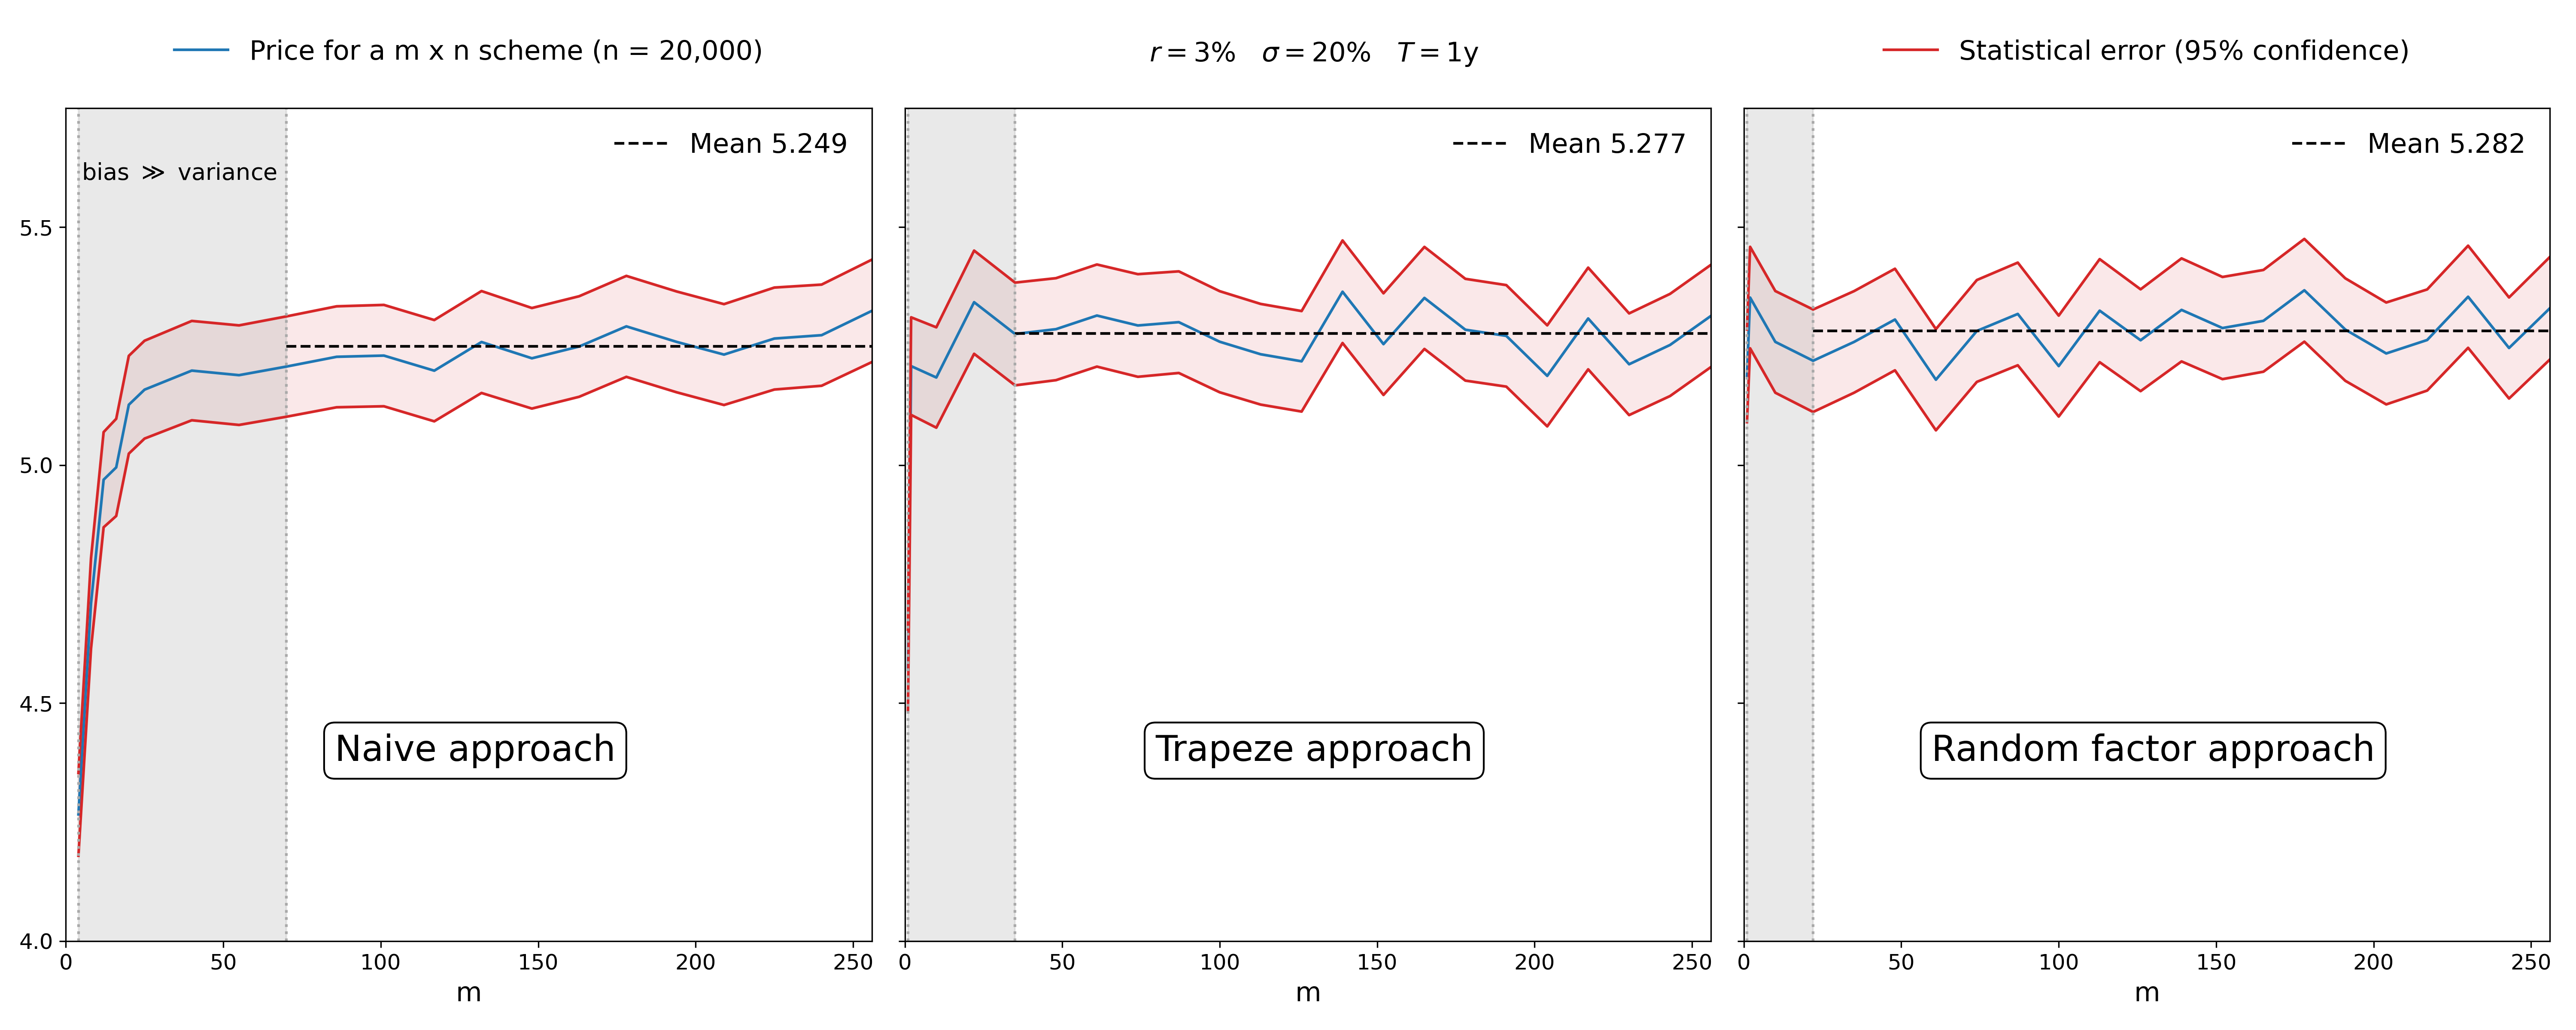
\includegraphics[width=1.04\textwidth]{charts/cvgce_wo_control.png}
  \caption{Convergence of schemes (1)-(3) for different values of $m$}
\end{figure}

\

Figure 2 shows the $95\%$ confidence intervals given by the three methods for fixed $n$ and $m$
varying up to $256$. As we do not have an analytical solution, it is difficult to compare the impact of the variance and that
of the bias by comparing the error to the confidence intervals for different values of $m$. However, since the proposed
methods are asymptotically unbiased, the black dotted lines are good approximations of the solution and we
can compare the fluctuations of the blue line with the width of the confidence intervals, in red. In the grey area,
that is to say for low values of $m$, the bias is high compared to the variance. For greater values of $m$, a plateau
seems to be reached and the observed deviations are mainly caused by the variance (the bias becomes negligible).
Thus, these charts allow
to choose $m$: the one at the edge of the grey zone is the most computationally-effective one that offers a satisfactory
level of accuracy. As explained before, there is actually no point in choosing higher values of $m$ since the decrease in
the bias would be hidden by the variance. Consequently, one can already notice the advantage of the two improved
methods on the right-hand side in comparison with the naive approach: $m$ can be chosen to be significantly lower
while achieving as good results. They allow better time complexity. Note however that their space complexity is worse.
In particular, the third method requires to simulate an additional $n \times m$ matrix of independent, normally
distributed coefficients.

\subsection{The use of a control variate}

The two improvements introduced in the above tackle the bias, which they successfully reduce for low values of $m$.
In order to improve the convergence speed with respect to parameter $n$,
Lambert et al. \cite{main} finally propose a variance reduction technique
for the three schemes above. It uses a control variate as introduced by Kemna et al. \cite{Vorst}.

\begin{equation}
	\theta_n = \sum_{i=1}^n \left( e^{-rT} \left[ A_T^i - K \right]_+ + \beta \left( Z^i - \mathbb E [Z] \right) \right)
	\tag{$\ast$}
\end{equation}

Observing that $e^x \approx 1 + x$ and $\ln(1 + x) \approx x$ when $| x |$ is small,
the idea relies on the approximation:
\[
	A_T = \frac{1}{T} \int_0^T S_u du \approx \exp \left\{ \frac{1}{T} \int_0^T \ln S_u du \right\}
	= S_0 \exp \left\{ \frac{1}{T} \int_0^T \ln \frac{S_u}{S_0} du \right\}
\]
The equality on the right-hand side justifies the validity of such approximation: if $r$ and $\sigma$ are small,
$S_u$ can be expected to remain near $S_0$ and $\ln \frac{S_u}{S_0} \ll 1$.
Therefore, we would like to use the following as a control variate in the case of a fixed-strike Asian call:
\[
	Z
	= e^{-rT} \left[ S_0 \exp \left\{ \left( r - \frac{\sigma^2}{2} \right) \frac{T}{2} +
		\frac{\sigma}{T} \int_0^T W_u du \right\}
		- K \right]_+
\]

Note that we can indeed compute the exact expression of $\mathbb E[Z]$. First, It\^o's lemma
gives $d(tW_t) = tdW_t + W_tdt$ and:

\[
	\frac{1}{T} \int_0^T W_u du = \frac{1}{T} \int_0^T (T-s) dW_s \sim \mathcal N \left(0, \frac{T}{3} \right)
	\quad \text{because} \quad \int_0^T (T-s)^2 ds = \frac{T^3}{3}
\]

If we note $a := \left( r - \frac{\sigma^2}{2} \right) \frac{T}{2}$, $b := \sigma \sqrt{\frac{T}{3}}$, $\rho :=\frac{K}{S_0}$,
$x^\ast := \frac{\ln \rho - a}{b}$ and $N$ the c.d.f of $\mathcal N (0, 1)$ then:
\begin{align*}
	\frac{\mathbb E[Z]}{e^{-rT} S_0}
	&= \int_{x^\ast}^{+ \infty} \left( e^{a + bx} - \rho \right) N'(x) dx \\
	&= e^{a + \frac{b^2}{2}} \int_{x^\ast - b}^{+ \infty} N'(u) du - \rho \int_{x^\ast}^{+ \infty} N'(x) dx
	\quad \text{with} \quad u = x - b \\
	&= e^{a + \frac{b^2}{2}} N(b - x^\ast) - \rho N(-x^\ast)
\end{align*}
	
On can check that the same computations yield Black-Scholes formula for the price of a European call.
Thus, we have the analytical expression. We finally need to provide a way to simulate the control variate $Z$
in each scenario. We define:

\begin{equation}
	\bar Z^{r, m} = e^{-rT} \left[ S_0 \exp \left\{ \left( r - \frac{\sigma^2}{2} \right) \frac{T}{2} +
		\frac{\sigma}{m} \sum_{i=0}^{m-1} \bar W_{t_k}^m \right\} - K \right]_+
	\tag{$i$}
\end{equation}

Plugging $\bar A_T^{r, m}$ from scheme $(1)$ and $\bar Z_T^{r, m}$ in $(\ast)$ yields a new estimator:
\begin{equation}
	e^{-rT} \left[ \bar A_T^{r, m} - K \right]_+ + \hat\beta_r \left( \bar Z_T^{r, m} - \mathbb E [Z] \right)
	\tag{4}
\end{equation}
where $\hat\beta_r$ is estimated with the empirical covariance of the variables.

\begin{figure}[H]
  \hspace*{-0.1\linewidth}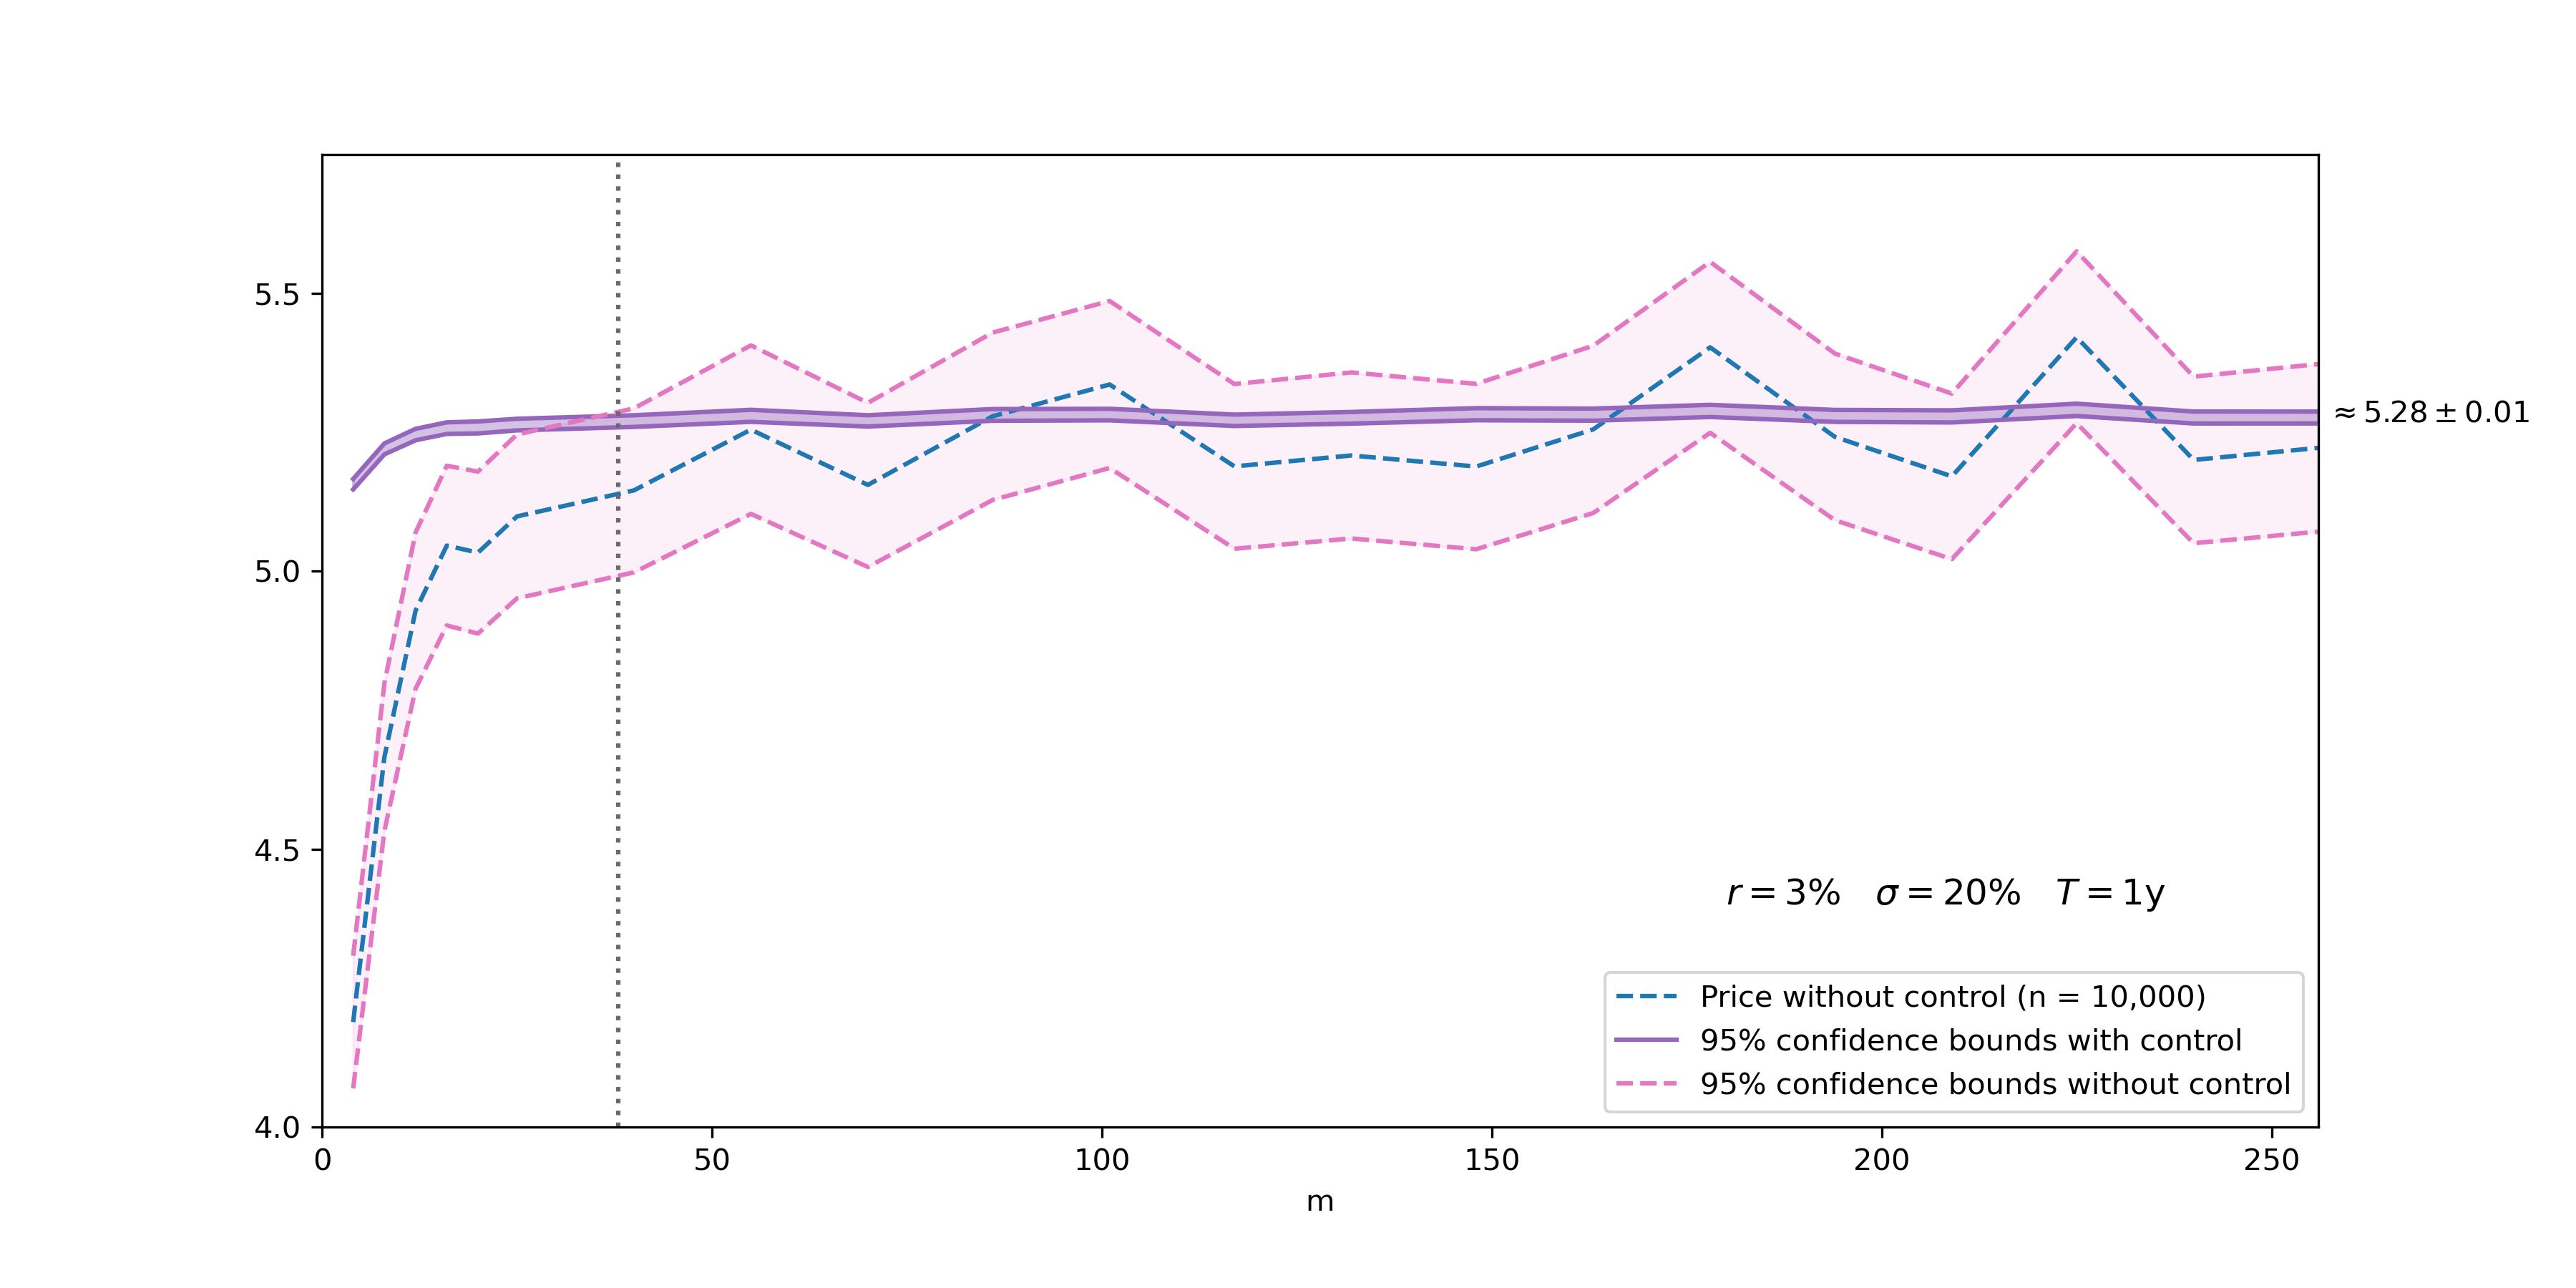
\includegraphics[width=1.1\textwidth]{charts/cvgce_control.png}
  \caption{Convergence of scheme (4) for different values of $m$}
\end{figure}

As expected, the statistical error (ie: the width of the confidence interval) is much more narrow. With this set of
parameters, it is about ten times smaller. The result is quite impressive. Besides, it does not only allow to take
a lower $n$ with better results but also to use a lower $m$. However, considering the assumptions this method relies on,
one could wonder whether this variance reduction technique is still as efficient when the parameters
($r$, $\sigma$ or $T$ for instance) are high. We testes this scheme for degenerate parameters and obtained really
satisfactory results: when $\sigma = r = 50\%$, the variance when using a control variate is still divided by 4
compared to the naive scheme (1).

\

The enhancement allowed by the control variate looks more interesting than the the one yielded by replacing
scheme (1) by scheme (2) or (3). Hopefully, it is possible to combine these improvements in order to obtain really
satisfactory results for both low values of $m$ and moderate values of $n$.

\subsection{The combination of both improvements}

As we did with scheme $(1)$, we can plug the estimates of schemes $(2)$ and $(3)$ in $(\ast)$. That requires
to adapt the estimates of $Z$ accordingly. Let us define:
\begin{equation}
	\bar Z^{e, m} = e^{-rT} \left[ S_0 \exp \left\{ \left( r - \frac{\sigma^2}{2} \right) \frac{T}{2} +
		\frac{\sigma}{m} \sum_{i=0}^{m-1} \frac{\bar W_{t_{k+1}}^m + \bar W_{t_k}^m}{2} \right\} - K \right]_+
	\tag{$ii$}
\end{equation}
\begin{equation}
	\bar Z^{p, m} = e^{-rT} \left[ S_0 \exp \left\{ \left( r - \frac{\sigma^2}{2} \right) \frac{T}{2} +
		\frac{\sigma}{m} \sum_{i=0}^{m-1} \bar J_k^m \right\} - K \right]_+
	\tag{$iii$}
\end{equation}

With (provided the same computations as for $\bar I_k^m$):
\[
	\bar J_k^m := \left( \frac{1}{h} \int_{t_k}^{t_{k+1}} \bar W_u du \ \Big\vert \ \bar W_{t_{k+1}}^m, \bar W_{t_k}^m \right)
	\sim \mathcal N \left( \frac{\bar W_{t_{k+1}}^m + \bar W_{t_k}^m}{2}, \frac{h}{12} \right)
\]

It yields two new estimators:

\begin{align}
	e^{-rT} \left[ \bar A_T^{e, m} - K \right]_+ + \hat\beta_e \left( \bar Z_T^{e, m} - \mathbb E [Z] \right)
	\tag{5} \\
	e^{-rT} \left[ \bar A_T^{p, m} - K \right]_+ + \hat\beta_p \left( \bar Z_T^{p, m} - \mathbb E [Z] \right)
	\tag{6}
\end{align}

\noindent Where $\hat\beta_e$ and $\hat\beta_p$ are still estimated with the empirical covariance of
$\bar Z_T^{e, m}$ (resp. $\bar Z_T^{p, m}$) and $\bar A_T^{e, m}$ (resp. $\bar A_T^{p, m}$). In practice, these two
schemes yield expected results, meaning they merge the advantages of scheme (2) (resp. (3)) and those of
the control variate observed with scheme (4). Undoubtedly, estimator (4) is the best one we have implemented so far.

\subsection{A possible step further}

Among the six schemes we have introduced, a great advantage of the third scheme (in particular compared to the
second one) is that it can be extended to other diffusion processes, while keeping the same convergence rate.
\begin{equation}
    A_T \approx \frac{1}{m} \sum_{k=0}^{m-1}
    	\bar S_{t_k}^m \left\{ 1 +
		\left( \frac{1}{h} \int_{t_k}^{t_{k+1}} \left( S_u - S_{t_k} \right) du \ \Big\vert \ \mathcal B_h \right) \right\} \tag{3+}
\end{equation}

This would for instance allow to use stochastic volatility models as long as the conditional integral can be simulated.
This is a very important aspect in order to better model the actual stock markets.
Unfortunately, it is not straight-forward to adapt the variance reduction technique as it strongly relies on
Black-Scholes model and consequently, the closed-form solution of an integral.

\section{PDE approaches}

\subsection{Mathematical background}

In the general case, it is possible to evaluate the price of an option if it satisfies a PDE.
Therefore, finding the price of the option is equivalent to solving a PDE.
To start with, we introduce the mathematical background and a well-chosen transformation as developed 
in \cite{Rogers} that satisfies a simple PDE.
As usual when it comes to pricing an option based on PDE's model, we define

\begin{equation}
	\phi(t,x) = \mathbb E \left[ \left[ \int_{t}^{T} \frac{S_{t}}{T}\,dt-x \right]_{+} \ \big\vert \ S_{t}=1 \right]
	\tag{I}
\end{equation}

The goal is to find a PDE satisfied by $\phi$. Let us define $M$ a well-chosen martingale.
Using It\^o's forumla:

\begin{align*}
        M_{t} &= \mathbb E \left[ \left[ \int_{0}^{T} \frac{S_{u}}{T}\,du-K \right]_{+} \ \Big\vert \ F_{t} \right] \\
        M_{t} &= \mathbb E \left[ \left[ \int_{t}^{T} \frac{S_{u}}{T}\,du+\int_{0}^{t} \frac{S_{u}}{T}\,du-K \right]_{+}
        	 \ \Big\vert \ F_{t} \right]  \\
        M_{t} &= S_{t} \mathbb E \left[ \left[ \int_{t}^{T} \frac{S_{u}}
        {TS_{t}}\,du -\frac{K-\int_{0}^{t} \frac{S_{u}}{T}\,du}{S_{t}} \right]_{+} \ \Big\vert \ F_{t} \right] \\
        M_{t} &= S_{t}\phi(t,\zeta_{t})
\end{align*}

Where
\[
	\zeta_{t} := \frac{K-\int_{0}^{t} \frac{S_{u}}{T}\,du}{S_{t}}
\]

Then, differentiating with respect to It\^o's formula and using the fact that $M_{t}$ is a martingale,
the following term in $dt$ must vanish:

\begin{equation}
	dM={c}{{S\left[r\phi+\dot{\phi}-\left(\rho_{t}+r\xi\right)\phi^{\prime}
	+\frac{1}{2}\sigma^{2}\xi^{2}\phi^{\prime\prime}\right]}}dt +...dW_t
	\tag{II}
\end{equation}

Then writing $f$ the discounted value of the price $\phi$ such that $f(x,t)=\exp(-r(T-t))\phi(x,t)$ \\
and replacing $f$ in (II) gives a simple PDE for $f$:

\begin{equation}
	\dot{f} + Gf=0
	\tag{PDE}
\end{equation}

With $G$ the operator such that
$G\equiv\frac{1}{2}\sigma^{2}x^{2}\frac{\partial^{2}}{\partial x^{2}}-(\rho_{t}+r x)\frac{\partial}{\partial x}$.
\\

It is also important to get the boundary conditions at time $T$. The initial definition of $\phi$ from (I)
in which the integral vanishes at time $t=T$ provides:
\[
	f(T,x)=(-x)_{+} 
\]

The previous transformation was useful because it helped finding a simple PDE for $f$.
What is more, the price of the Asian option with a fixed strike $K$ is given by:
\[
 	e^{-r T} \mathbb E \left[ \left[ \int_{0}^{T} \left( S_{u}-K \right) \frac{du}{T} \right]^{+} \right]
	=S_{0} f \left( 0, K S_{0}^{-1} \right) \equiv e^{-r T} S_{0} \phi \left( 0, K S_{0}^{-1} \right)
\]

Hence, solving the PDE and obtaining the values of $f$ at time $t=0$ allows to estimate the price of the option.
It is possible to solve numerically this linear equation with a classic finite difference method. 

\subsection{Solving the PDE}

In this section, we solve the following PDE thanks to numerical finite difference method:

\[
	\begin{cases}
		\dot{f} + Gf = 0 \\
		f(T,x)=(-x)_{+}
	\end{cases}
	\quad \text{with} \qquad
	G \equiv \frac{1}{2}\sigma^{2}x^{2}\frac{\partial^{2}}{\partial x^{2}}-(\rho_{t}+r x)\frac{\partial}{\partial x}
\]

To compute the price, we use an explicit scheme:
\[
	\frac{u_{i}^{n+1} -u_{i}^{n}}{h} \approx \frac{d}{dt} u(t_n,x_i)\approx -Gu^{n}
\]

\subsection*{Parameters used}

Some parameters are fixed during each simulation:

\begin{itemize}[label=$\cdot$]
    \item $\sigma\in{0.15;0.25}$ the volatility is taken constant
    \item $r=0.03$ the interest rate is constant 
    \item $T=1$ the maturity
    \item $x\in[-5;5]$ 
\end{itemize}

The space and the time are discretized with  space step $\delta \approx 2.10^{-3}$ and time step $h \approx 10^{-3}$.
The space step should not be too small with respect to time otherwise it could lead to some instabilities or unsatisfactory
results. Intuitively as the initial conditions at $t=T$ vanishes (ie: $\phi(T,x) = 0$ for $x > 0$),
the operator $G$ (proportional to the derivatives of $f$) takes higher number of time iterations $t_i$
to reach and impact $\phi(t_i,.)$ on the whole positive domain $x>0$.
\\

The results as shown in Figure 4 are satisfactory in the sense that they are consistent with what we obtained
with the Monte Carlo approaches. 
\begin{figure}[h]
  \centering
  \begin{minipage}{0.45\textwidth}
    \centering
    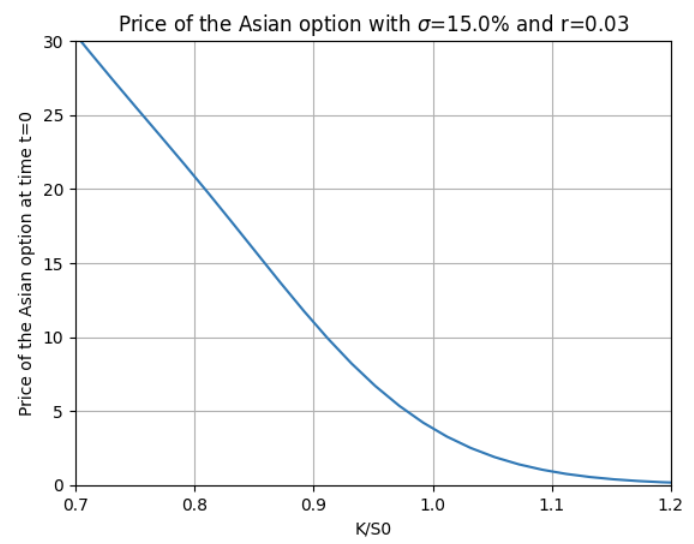
\includegraphics[width=\textwidth]{charts/Price_alone15.png}
  
  \end{minipage}\hfill
  \begin{minipage}{0.45\textwidth}
    \centering
    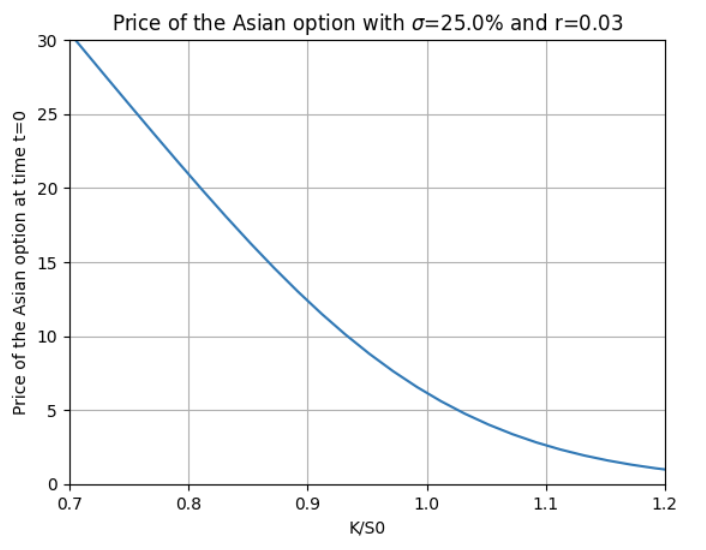
\includegraphics[width=\textwidth]{charts/Price_alone_25.png}
    
  \end{minipage}
  \caption{Price curves with respect to the strike with the PDE approach}
\end{figure}

\section{Lower and upper bounds for the computed price}

Computing numerically a price is not enough to have a correct estimation. It is also important to tackle the errors
due to the numerical method and thus to find bounds to be able to judge the reliability of the result.
In that case, we look for a lower bound for the price that we can establish theoretically and then compute it.
Once more, the main ideas of this section were already developed in \cite{Rogers}.

\subsection{Theoretical approach}
Let $\operatorname{\mathbb{E}}[Y^{+}]$ denotes the price of the Asian option that we want to bound. For any centered Gaussian variable $Z$, we get:
\begin{equation}
\operatorname{\mathbb{E}}[Y^{+}]=\operatorname{\mathbb{E}}[\operatorname{\mathbb{E}}[Y^{+}\mid Z]]\geq\operatorname{\mathbb{E}}\left[\operatorname{\mathbb{E}}[Y\mid Z]^{+}\right]
\tag{III}
\end{equation}
 
What is more, for any random variable $U$:

 \begin{equation}
    \begin{aligned}
    &0\leq \mathbb{E}[U^{+}]-\mathbb{E}[U]^{+} \\ 
    &{{\leq\,\frac{1}{2}(\mathbb{E}[|U|]-\,|\mathbb{E}[U]|)}}\\ 
    &{{\leq\,\frac{1}{2}\mathrm{var}[U]^{1/2}.}}
    \end{aligned}
    \tag{IV}
 \end{equation}
 Hence combining (III) and (IV) provides a framework for the price:

\[
\mathbb{E}[\mathbb{E}[Y\mid Z]^{+}]\leq \mathbb{E}[Y^{+}] \leq \mathbb{E}[\mathbb{E}[Y\mid Z]^{+}] + \frac{1}{2}\mathbb{E}[\mathrm{Var}[Y^{+}\mid Z]^{1/2}]
\]

The purpose of this inequality is to find a well-chosen $Z$ which minimizes $\mathbb{E}[\mathrm{Var}[Y^{+}\mid Z]^{1/2}]$ to frame the price at best. We are looking for a normally distributed variable so that:
\begin{align*}
  &\mathbb{E}[B_t\mid Z]=m_{t}Z\\
  &\mathrm{Cov}(B_s,B_t\mid Z)=v_{st} 
\end{align*}

As in the numerical tests, we choose $T=1$. That explains the bounds of the following integrals.
The goal is now to compute $\mathrm{Var}[Y^{+}\mid Z]^{1/2}$.
As a first step, we should compute the mean of $Y^{+} \mid Z$.
Quoting the article, \textit{it turns out that choosing the following definition of $Z$ is by far the best choice}.
\[
   	Z := TA_T = \int_{0}^{T} S_{t} \,dt 
\]

Adopting this definition yields:
\[
\mathbb{E}[Y\mid Z]=\mathbb{E}\left[\int_{0}^{1}\exp(\sigma B_{t}-{\textstyle\frac{1}{2}}\sigma^{2}t+r t)\,dt
\ \Big\vert \ Z \right]=\int_{0}^{1}\exp(\sigma tZ-{\textstyle\frac{1}{2}}\sigma^{2}v m_{t}^{2}+r t)dt
\]

Where $v=Var(Z)$. After some calculations:
\[
\mathrm{Var}[Y\mid Z]=\int_{0}^{1}d s\int_{0}^{1}\exp(\sigma Z(m_{s}+m_{t})-{\textstyle{\frac{1}{2}}}\sigma^{2}v(m_{s}^{2}+m_{t}^{2})+r(s+t))(e^{\sigma^{2}v_{s t}}-1)d t
\]

For common values of $\sigma$ (usually $\in[0.03;0.6]$) and provided that for $s,t \in [0,1]$:
\[
	| v_{st} | = | \mathrm{Cov} (B_s,B_t\mid Z)| \leq \mathrm{Var}(B_s)^{\frac{1}{2}} Var(B_t)^{\frac{1}{2}}\leq 1
\]
we can simplify the above expression using $e^{\sigma^{2}v_{s t}}-1\approx \sigma^{2}v_{s t}$\\
\\
This approximation is then used to approximate the integral giving $\mathrm{Var}[Y\mid Z]$.
As a result, we define the approximate integral $V$:
\begin{align*}
	V &\approx \int_{0}^{1} ds\int_{0}^{1}(1+\sigma Z(m_{s}+m_{t})-{\textstyle\frac{1}{2}}
	\sigma^{2}v(m_{s}^{2}+m_{t}^{2})	+r(s+t))\sigma^{2}v_{s t}d t \\
	&=\int_{0}^{1}ds\int_{0}^{1} (1+f(s,Z)+f(t,Z))v_{s t}dt
\end{align*}
where $f(t,Z)=\textstyle\frac{1}{2}\sigma^{2}v(m_{t}^{2}+rt)\sigma^{2}$.
\\

The noticeable thing about this integral is to observe that it vanishes when $Z=\int_{0}^{1}B_u du$\\
Indeed, by bilinearity of the covariance:\\
\begin{equation}
    \int_{0}^{1}v_{st}ds=\int_{0}^{1}cov(B_s,B_t\mid Z)ds=cov(\int_{0}^{1}B_s ds,B_t\mid Z)=cov(Z,B_t\mid Z)=0
\end{equation}
As a consequence, we just found an ideal candidate for $Z$ : assuming that the initial integral $\mathrm{Var}[Y\mid Z]$ is close to $V$, vanishing $V$ implies reducing significantly $\mathrm{Var}[Y\mid Z]$.\\
With $Z$ vanishing $V$:
\begin{equation}
  \mathrm{Var}[Y\mid Z]= \mathrm{Var}[Y\mid Z]-V\leq A+B 
\end{equation}
Where 
\begin{equation}
    \begin{aligned}
    &A=\int_{0}^{1}d s\int_{0}^{1}\ (e^{f(s,Z)+f(t,Z)}-1-f(s,Z)-f(t,Z)).|e^{\sigma^{2}v_{s t}}-1|d t\\
    &B=\int_{0}^{1}d s\int_{0}^{1}(e^{\sigma^{2}v_{s t}}-1-\sigma^{2}v_{s t}).|1+f(s,Z)+f(t,Z)|d t
    \end{aligned}
\end{equation}
After some computations detailed in [3], we finally get
\begin{equation}
    \mathbb{E}[\mathrm{Var}[Y^{+}\mid Z]^{1/2}] \leq \frac{1}{2}\Biggl[c\sigma^{2}e^{c\sigma^{2}+\gamma_{2}}\biggl[\frac{1}{2}\sigma^{2}\gamma_{1}v e^{{\frac{1}{2}}\sigma^{2}\gamma_{1}v}+{\textstyle{\frac{1}{2}}}\gamma_{2}^{2}\biggr]+{\textstyle{\frac{1}{2}}}\sigma^{4}c^{2}e^{\sigma^{4}c^{2}}(1+\gamma_{2})\Biggr]^{1/2}
\end{equation}
Where 
\begin{equation}
    |v_{s t}|\leq c,\ \ \ (m_{s}+m_{t})^{2}\leq\gamma_{1},\ \ \ |g_{s}+g_{t}|\leq\gamma_{2} ,\ \ \ 
    g_s\equiv r s-\textstyle{\frac{1}{2}}\sigma^{2}v m_{s}
\end{equation}
It is then necessary to find optimal parameters minimizing the right-term of (18). \\
As $Z=\int_{0}^{1}B_u du$, we deduce that $v=\frac{1}{3}$.

\subsection{Computation of the theoretical bounds}

Thanks to the preceding part, we should be able to compute a lower and upper bounds. 

Indeed, for a strike $K$, the price $\mathbb{E}[(Y-K)_{+}]$ is framed by by:
\begin{equation}
    \mathbb{E}[\mathbb{E}[(Y-K)\mid Z]_{+}]\leq \mathbb{E}[(Y-K)_{+}] \leq  \mathbb{E}[\mathbb{E}[(Y-K)\mid Z]_{+}]+Var[Y\mid Z]^{1/2} \leq \mathbb{E}[\mathbb{E}[(Y-K)\mid Z]_{+}]+A+B 
\end{equation}
With $A+B$ majored in (18).\\
We first need to compute the lower bound
\subsection{Computing the lower bound}
In this part, we compute $\mathbb{E}[\mathbb{E}[(Y-K)\mid Z]_{+}]$ with $Z=\int_{0}^{1}B_u du$ and $Z \sim \mathcal{N}(0,\frac{1}{3})$.\\
To start with\\

\begin{equation}
 \begin{aligned}
     &\mathbb{E}[(Y-K)\mid Z]=\phi(Z) \\
     &With:\\
     &\mathbb{E}[(Y-K)\mid Z=z]=\phi(z)
 \end{aligned}
\end{equation}
Then, using (12) we find:

\begin{equation}
\phi(z)=-K+\int_{0}^{1}\exp(\sigma tz-{\textstyle\frac{1}{2}}\sigma^{2}v m_{t}^{2}+r t)dt
\end{equation}
And taking into account the density of Z $f_Z(x)=\frac{3}{\sqrt{2\pi}} \cdot e^{-\frac{3x^2}{2}}$\\
We finally find:\\
\begin{equation}
\mathbb{E}[\mathbb{E}[(Y-K)\mid Z]_{+}]=\int_{-\infty}^{+\infty}\phi_{K}(x)_{+}f_Z(x)dx
\end{equation}
This last integral can easily be estimated with the python scipy module.

\subsection{Computing the upper bound}

In fact, computing the upper bound is quite simple as we only need to add to the lower bound this quantity:\\
$\frac{1}{2}\Biggl[c\sigma^{2}e^{c\sigma^{2}+\gamma_{2}}\biggl[\frac{1}{2}\sigma^{2}\gamma_{1}v e^{{\frac{1}{2}}\sigma^{2}\gamma_{1}v}+{\textstyle{\frac{1}{2}}}\gamma_{2}^{2}\biggr]+{\textstyle{\frac{1}{2}}}\sigma^{4}c^{2}e^{\sigma^{4}c^{2}}(1+\gamma_{2})\Biggr]^{1/2}$\\
\\
With well-chosen parameters satisfying (19):\\
\begin{equation}
    c=\frac{1}{3}\ \ \ 
    \gamma_{1}=9\ \ \ 
    \gamma_{2}=r+\frac{\sigma^{2}}{4} 
\end{equation}

We finally get really convincing results close to the PDE solution computed previously.\\ 
Notice that the bounds are not supposed to directly frame the PDE solution computed but only the price in the general case. However, we could estimate an upper bound of the relative error conveyed by the PDE solution thanks to these bounds. \\
\begin{figure}[h]
  \centering
  \begin{minipage}{0.5\textwidth}
    \centering
    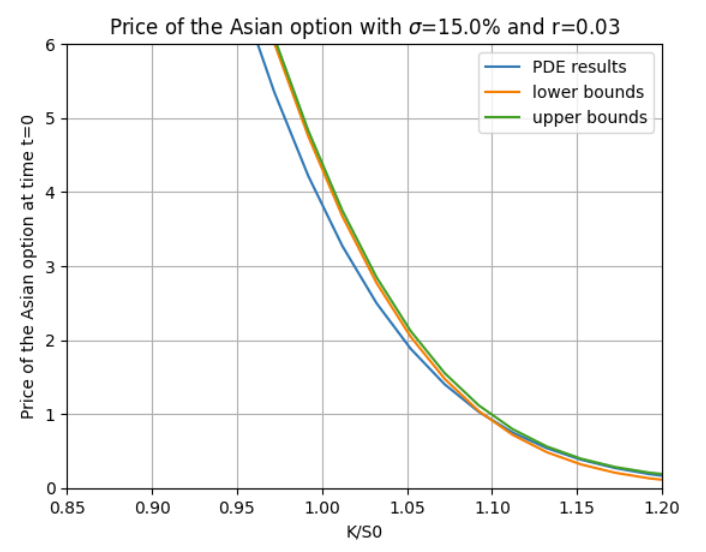
\includegraphics[width=\textwidth]{charts/Pric_bounds15.png}
    
  \end{minipage}\hfill
  \begin{minipage}{0.5\textwidth}
    \centering
    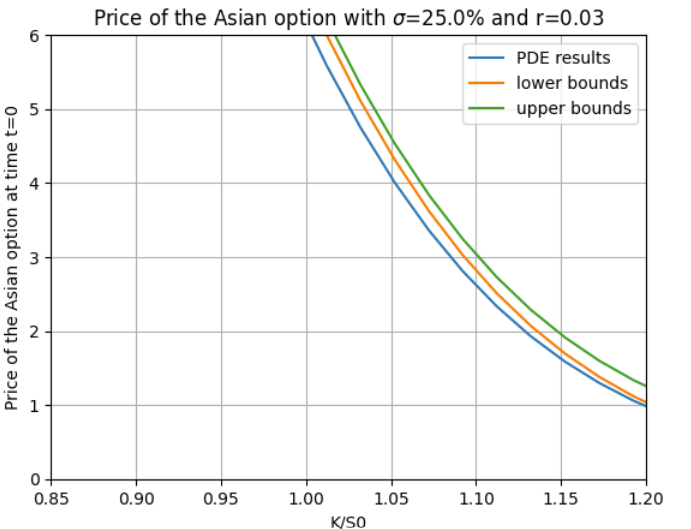
\includegraphics[width=\textwidth]{charts/Price_bounds25.png}
   
  \end{minipage}
\end{figure}
\section{Convergence analysis}
The Monte-Carlo course (section 2.3 of chapter 7) gives an easy way to check theoretically the convergence of an explicit scheme (case $\theta=0$). Hence, assuming there exists a smooth solution to the PDE, if
\begin{equation}
    |b(x_i)|\delta\leq \sigma^{2}(x_i), \\\
    \sigma^{2}(x_i)h\leq \delta^{2}
\end{equation}
Where $\delta$ is the space step and $h$ is the time step.\\
Then the scheme is convergent for the $L_\infty $ norm.\\
In our practical cases, this last equation is equivalent to these inequalities:
\begin{equation}
    \begin{aligned}
        &0\leq \frac{\sigma^{2}x_i^{2}}{2}-|\rho_t+rx_i|\delta, \\
        &0\leq \delta^{2}- \frac{\sigma^{2}x_i^{2}}{2}h
    \end{aligned}
\end{equation}
Here, $\delta \approx 2.10^{-3}$ and $h \approx 10^{-3}$.\\
We plot these inequalities for two values of $\sigma$.  We could also play with the step parameters $\delta$ and $h$ to ensure that these two functions remains positive.
\begin{figure}[h]
  \centering
  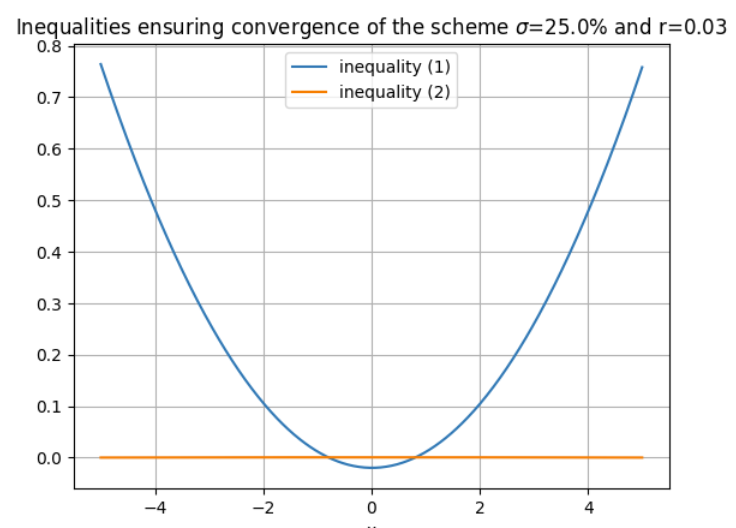
\includegraphics[width=0.8\textwidth]{charts/Ineq.png}
\end{figure}
\subsection{Critics of the convergence proof }
Graphically, the results are not really convincing, however the inequalities are in both cases almost verified in the whole domain and it is enough for us to observe convergence.\\
Moreover, we observe that issues of convergence could especially occur around 0, while inequalities seem to be verified on the edges.\\ 
It would be also possible to study more in detail the stability and the consistency of the explicit scheme used to give better arguments to justify the convergence for a wide range of  parameters.\\

\section*{Conclusion}

\renewcommand{\arraystretch}{1.2}

\begin{center}
\begin{tabular}{m{0.25\textwidth}>{\centering}m{0.15\textwidth}>{\centering}m{0.15\textwidth}
	>{\centering\arraybackslash}m{0.3\textwidth}}
    \hline
    	\multirow{2}{*}{\textbf{Method}} &
   	\multicolumn{2}{c}{\textbf{Results}} &
	\multirow{2}{*}{\textbf{Processing time (s)}} \\
	\cline{2-3} & \textbf{Value} & \textbf{Interval} & \\
    \hline
    $\text{MC}_1$ (naive) & & & \\
    $\text{MC}_2$ (trapeze)  & & &  \\
    $\text{MC}_3$ (conditional)  & & & \\ %\multicolumn{2}{c}{content}
    $\text{MC}_1$ (+ control) & & & \\
    $\text{MC}_2$ (+ control)  & & & \\
    $\text{MC}_3$ (+ control)  & & & \\
    PDE approach & & \textit{NA} & \\
    Lower-upper bounds & & & \\
    \hline
\end{tabular}
\end{center}


\bibliography{bibliography}{}
\bibliographystyle{plain}

\end{document}
